\section{Results and Analysis}

\subsection{Core Recommendation Metrics}

Fig.~\ref{fig:core_metrics} shows the performance of different models across multiple interaction stages (T0, T100, T300, T500).
These stages represent how the system behaves as more user interaction history becomes available.

\begin{figure*}[!h]
\centering
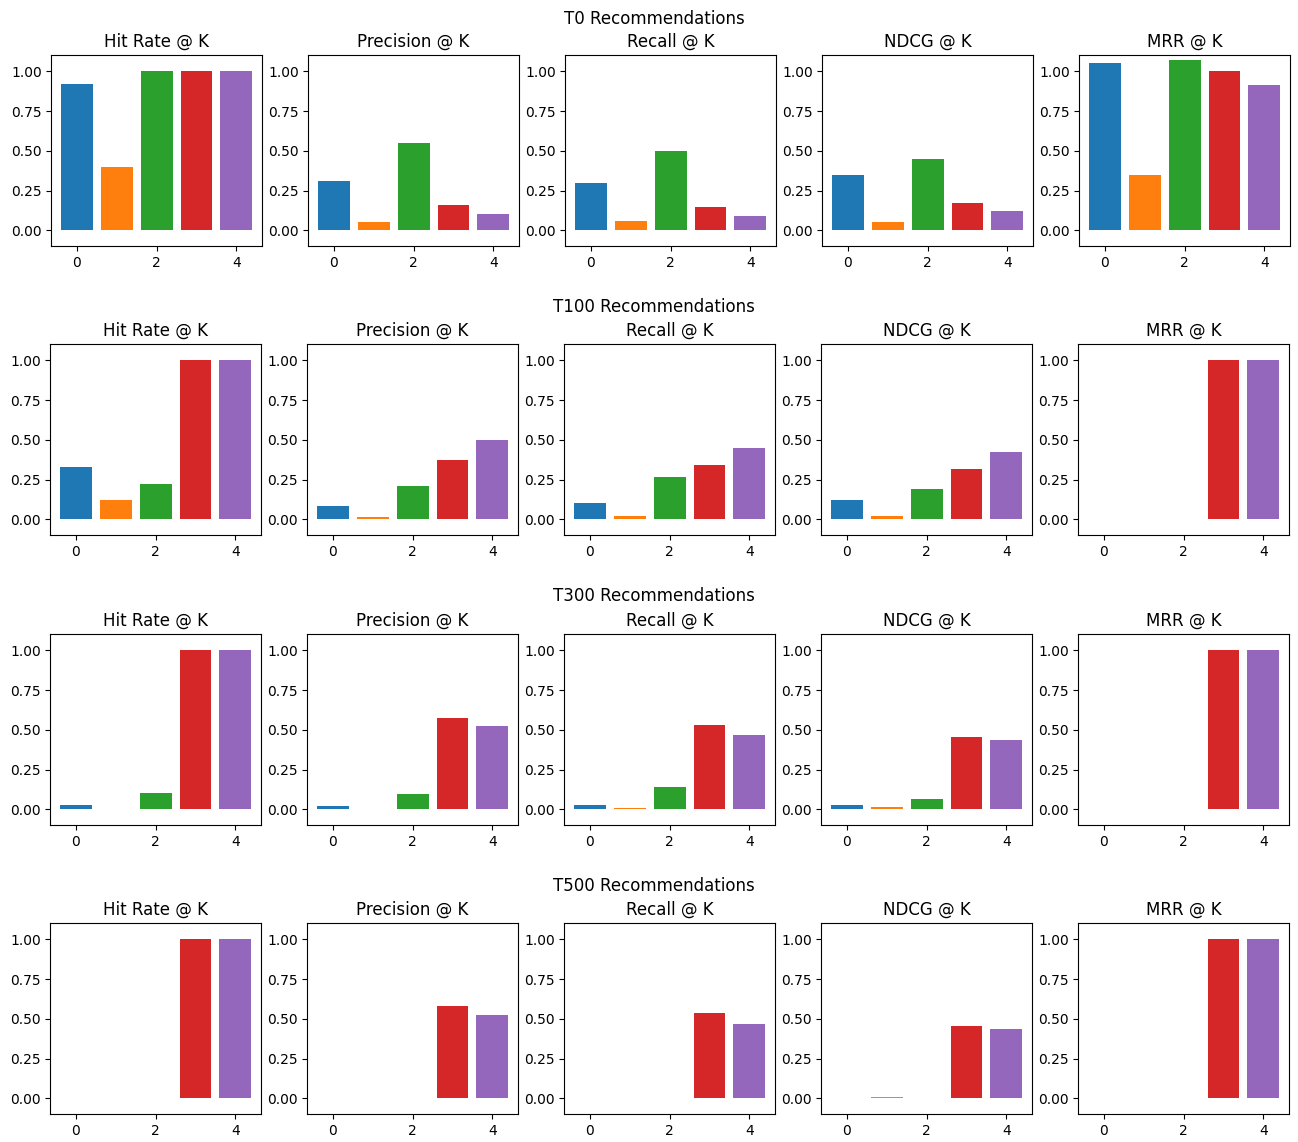
\includegraphics[width=\textwidth]{../figures/core metrics.png}
\caption{Performance comparison of all models across different interaction stages (T0, T100, T300, T500). Static models such as ALS and S1 perform well at early stages but degrade as user preferences evolve. In contrast, S2P and S2F improve over time by adapting to interaction history, with S2F showing a slight trade-off in accuracy due to cognitive-state-aware recommendations.}
\label{fig:core_metrics}
\end{figure*}

\subsubsection{Performance at Initial Stage (T0)}

At T0, where no interaction history is available, the \textbf{S1 model performs the best across all accuracy and ranking metrics}. 
This is expected, since S1 is trained on static user preferences and is specifically designed for this scenario.

On the other hand, both \textbf{S2P and S2F perform relatively poorly at this stage}.
These models rely on interaction history to update user preferences,
and in the absence of such history, they do not have enough information to perform well.

This shows that \textbf{static models are strong in cold-start or early-stage scenarios}.

\subsubsection{Effect of Preference Dynamics (T100 to T300)}

As interaction history increases, a clear shift in performance can be observed.

The performance of \textbf{S1 drops significantly} across all metrics. 
This indicates that static embeddings quickly become outdated when user preferences start evolving.

In contrast, \textbf{S2P shows a strong improvement} in all metrics. 
Since it updates user embeddings using interaction history, it is able to track preference changes effectively. 
As a result, it outperforms all static and classical models in mid and later stages.

This demonstrates the importance of \textbf{modeling preference dynamics instead of relying on fixed embeddings}.

\subsubsection{Effect of Cognitive Modeling (S2P vs S2F)}

When comparing S2P and S2F, an interesting pattern emerges.

S2P achieves \textbf{slightly higher values in precision, recall, and NDCG}, indicating that it is more focused on recommending highly relevant items.

However, S2F performs slightly lower on these metrics. 
This is expected, since S2F does not purely optimize for relevance. 
Instead, it balances:

\begin{itemize}
    \item Relevance
    \item Fatigue
    \item Discontentment
\end{itemize}

Because of this, S2F occasionally introduces less relevant or more diverse items, which slightly reduces short-term accuracy.

This highlights an important trade-off:

\textbf{Optimizing only for relevance (S2P) leads to better short-term accuracy, while incorporating cognitive factors (S2F) leads to more balanced and sustainable recommendation behavior.}

\subsubsection{Long-Term Behavior (T300 to T500)}

At later stages, both S2P and S2F achieve very high performance, with:

\begin{itemize}
    \item Hit Rate approaching 1
    \item MRR close to 1
\end{itemize}

This means that \textbf{relevant items are almost always present, and often appear at the top of the recommendation list}.

Meanwhile, S1 continues to degrade, and classical methods like ALS and BPR fail to adapt to changing preferences.

This further reinforces that:

\textbf{Static and traditional models are not suitable for dynamic recommendation environments.}


%%%%%%%%%%%%%%%%%%%%%%%%%%%%%%%%%%%%%%%%%%%%%%%%%%%%%%%%%%%%%%%%
%%%%%%%%%%%%%%%%%%%%%%%%%%%%%%%%%%%%%%%%%%%%%%%%%%%%%%%%%%%%%%%%

\subsection{Simulation Metrics}

The second set of results focuses on the simulated behavior of the user, rather than only the ranking quality of the recommender. 
These metrics are important because our system is not just trying to recommend relevant items. 
It is also trying to control fatigue, avoid discontentment, and keep the interaction healthy over time. 
Fig.~\ref{fig:simulation_metrics} shows four key behavioral metrics: return rate, acceptance rate, time to boredom, and coverage.

\begin{figure*}[!h]
\centering
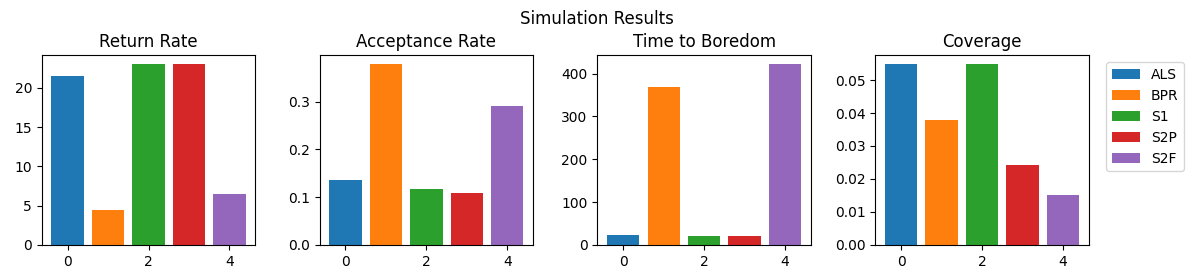
\includegraphics[width=\textwidth]{../figures/simulation metrics.png}
\caption{Comparison of behavioral metrics including return rate, acceptance rate, time to boredom, and coverage. While relevance-driven models (ALS, S1, S2P) lead to quicker fatigue, S2F significantly increases time to boredom by balancing relevance and diversity. The coverage trends highlight the interaction between recommendation behavior and evolving user preference within the simulation.}
\label{fig:simulation_metrics}
\end{figure*}

\subsubsection{Behavioral Trade-offs Across Models}

A clear pattern appears in the \textbf{return rate} and \textbf{time to boredom} plots.
The classical models, \textbf{ALS} and \textbf{S1}, show a relatively high return rate and a low time to boredom. 
This suggests that these models often keep recommending items that are relevant enough to trigger interaction, 
but also repetitive enough to make the user tired fairly quickly. 
In other words, they are able to engage the user, but they do not manage the experience very well over time.

\textbf{S2P} follows a similar pattern. 
Even though it updates the user preference using history, it is still strongly relevance-driven. 
Because of that, it can keep showing items that are close to the user's current interest, which is useful in the short term but can still lead to fatigue. 
This explains why S2P does not completely escape the "high relevance, quick boredom" behavior.

\textbf{S2F} behaves very differently. 
It has the \textbf{highest time to boredom} by a large margin, which is exactly what we would want from a cognitive-state-aware model. 
This means the user stays active for much longer before reaching fatigue. 
At the same time, its return rate is lower than the other strong models, which suggests that it is avoiding excessive overload and spreading the interaction more carefully. 
This is a good sign, because S2F is supposed to balance relevance with cognitive comfort, not just maximize clicks.

So overall, this plot supports the main idea of the project:
\textbf{pure relevance is not enough, and the best long-term system is the one that knows when to slow down.}

\subsubsection{Acceptance Rate Is Not the Full Story}

The \textbf{acceptance rate} plot is more subtle.

At first glance, \textbf{BPR} looks surprisingly strong here, even though it performs poorly on the core ranking metrics. 
This is a good reminder that acceptance rate alone does not tell the full story. 
Since it is averaged over time, it can be influenced by a few early clicks or by short periods where the model happens to align with the user's changing preference. 
So a high acceptance rate does not necessarily mean the model is actually good overall.

For \textbf{ALS}, \textbf{S1}, and \textbf{S2P}, the acceptance rate is lower than BPR, which may seem surprising at first. 
But this makes sense when we connect it with the earlier plots. 
These models are often producing highly relevant items, but they can also push the user toward fatigue faster. 
So the user may still click, but the interaction does not stay healthy for long.

\textbf{S2F} sits in the middle. 
Its acceptance rate is better than S1 and S2P, but lower than BPR. 
This is reasonable, because S2F is not only trying to get clicks. 
It is also trying to manage fatigue and discontentment. 
That makes it less aggressive, but more balanced.

The important takeaway is that \textbf{acceptance rate must be read together with ranking quality and time-based behavior}. 
On its own, it is too easy to misinterpret.

\subsubsection{Coverage and the Exploration Paradox}

The \textbf{coverage} plot is the most interesting one, and honestly, it reveals a very important limitation of the simulation setup.

At first, \textbf{ALS} and \textbf{S1} appear to have the highest coverage. 
\textbf{S2P} and \textbf{S2F} are lower, with S2F being the lowest. 
At face value, this seems strange, because we would normally expect dynamic models to explore more items. 
But in this simulator, coverage is not a completely fixed quantity. 
The set of "true" items is tied to the user's evolving preference, and that preference is shaped by the recommendations the user sees.

When a model shows a broader variety of items, the user preference can expand too, which enlarges the set of items considered relevant later on. 
So in this setup, a model that explores more can actually end up with a larger true-item space, which makes coverage look smaller.

This is why the result is not necessarily a bug in the model. 
It may actually be a sign that the simulator itself is capturing preference growth in a very strong way. 
In other words:

\begin{itemize}
    \item \textbf{ALS and S1} stay in a narrower region of the item space, so the true-item set remains smaller.
    \item \textbf{S2P and S2F} expose the user to a wider range of items, so the preference space grows, and coverage goes down relative to that larger set.
\end{itemize}

This is a very important point, because it means the coverage metric here is not just measuring "how much of the catalog was recommended." 
It is also measuring "how much the user's relevant space expanded during simulation." 
That makes it useful, but also harder to interpret.

A second reason this effect may be happening is that the simulation currently always takes the \textbf{first item from the top-k list} to continue the next step. 
That makes the trajectory more deterministic and may limit the exploration benefit of the broader top-k list. 
So the low coverage of S2P and S2F may partly come from the simulation policy itself, not only from the recommender.

\subsubsection{What We Learned from the Dropped Metrics}

Some of the other metrics did not contribute much extra information, so they were not emphasized in the final analysis.

The \textbf{content repetition rate}, \textbf{time to discontent}, and \textbf{serendipity} plots were almost flat across models, 
so they did not help distinguish the systems in a meaningful way. 
Likewise, the \textbf{fatigue score} was heavily dominated by the time-to-boredom term, so it behaved very similarly to that metric and did not add much new insight.

That is actually useful to know, because it tells us that not every metric is equally informative in this simulator. 
Some of them are redundant, while others are too sensitive to the current simulation design. 
So for the final discussion, the most meaningful behavioral signals are the ones that clearly separate the models: \textbf{return rate, acceptance rate, time to boredom, and coverage}.

\subsection{Summary of Key Observations}

The results highlight a few key points:

\begin{enumerate}
    \item \textbf{Static models work well only at the start.} \\
        They give good recommendations early, but struggle as user preferences change.
    \item \textbf{S2P improves performance over time.} \\
        It tracks changing preferences, but still focuses mainly on relevance, which can lead to user fatigue.
    \item \textbf{S2F offers a better balance.} \\
        It may slightly reduce short-term accuracy, but it delays boredom and supports longer, more stable interactions.
    \item \textbf{Classical models and S1 have weak long-term behavior.} \\
        They keep users engaged only for a short time before fatigue builds up.
    \item \textbf{Evaluation results should be interpreted carefully.} \\
        The simulated user changes based on the model’s recommendations, so some metrics are influenced by the model itself.
\end{enumerate}

Overall, these results suggest that recommendation systems should move beyond static predictions and consider both changing preferences and user behavior.
